\documentclass{standalone}
\usepackage{tikz}
\usetikzlibrary{shapes,arrows,positioning}
\begin{document}
  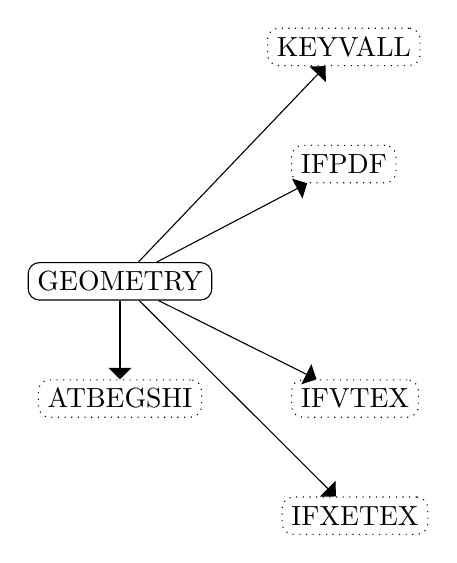
\begin{tikzpicture}
  \tikzset{main node/.style={rectangle, draw,
		text centered, rounded corners}, }
\tikzset{internal node/.style={rectangle, draw,dotted,
		text centered, rounded corners}, }
\tikzset{driver node/.style={ellipse, draw,dashed,
		text centered}, }
\tikzset{formato node/.style={rectangle, draw,dotted,
		text centered}, }
\tikzset{cfg node/.style={minimum size=1cm}, }
\tikzset{linea/.style={-triangle 90},}
    \node[main node] (1)   {GEOMETRY};
    %\node (2) [right =of 1]  {};
   \node[internal node] (3) [above right =of 1]   {IFPDF};
   \node[internal node] (4) [above =of 3] {KEYVALL};
   \node[internal node] (5) [below right =of 1]  {IFVTEX};
   \node[internal node] (6) [below =of 5] {IFXETEX};
   \node[internal node] (7) [below =of 1] {ATBEGSHI};
%
\foreach \x /\y in{1/3,1/4,1/5,1/6,1/7}
  \path[linea] (\x) edge node {} (\y);
%  
\end{tikzpicture}
\end{document}